\section{CFD Stability Tests}

In addition to the eigenvalue stability analysis discussed in the main
chapter, we performed numerical stability tests of the compact operators
using both Maxwell's equations and the BSSN equations. Representative
results from these tests are presented below.

For the Maxwell test, the computational domain extends over
$x,y,z\in[-20,20]$. We use the same initial data and numerical parameters
described in the computational fluid dynamics chapter and perform the
evolution on the corresponding low resolution uniform grid. The numerical
error remains bounded throughout the evolution and decreases cleanly after
the initial electromagnetic pulse propagates across the domain. We find no
evidence of growing numerical modes for any of the operators shown in
Fig.~\ref{fig:EM_all_operator_errors}.

\begin{figure}[htbp]
    \centering
    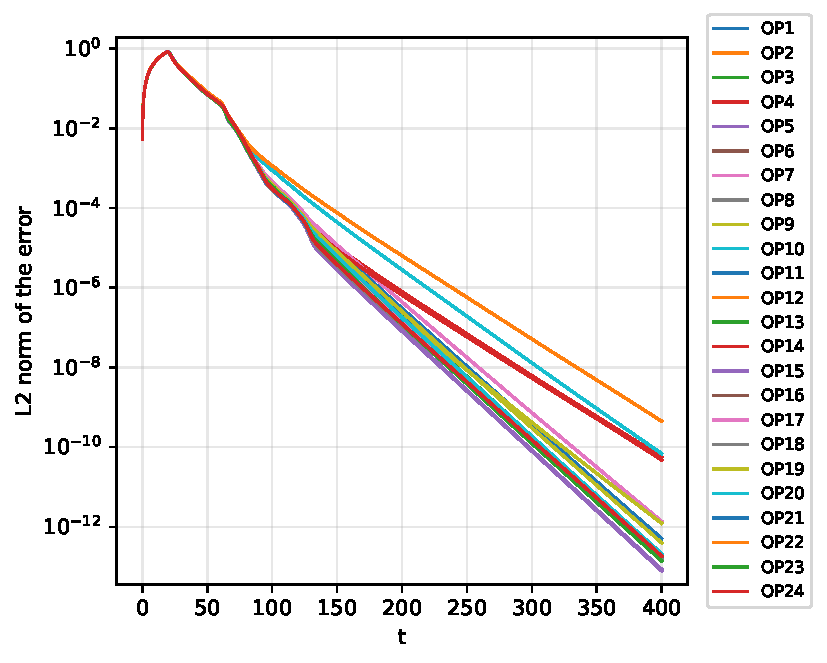
\includegraphics[width=0.9\textwidth]
    {Figures/Appendix/EM_all_operator_errors.pdf}
    \caption{
    Evolution of the numerical errors for the finite difference operators
    applied to the Maxwell test problem. The simulations use a uniform grid
    on the domain $x,y,z\in[-20,20]$ with the same initial data and numerical
    parameters used in the Maxwell tests presented in the main text. The
    errors remain bounded and decay cleanly as the electromagnetic pulse
    propagates out of the computational domain, with no evidence of a
    numerical instability.
    }
    \label{fig:EM_all_operator_errors}
\end{figure}

We also test the operators by evolving Teukolsky wave initial data with the
full BSSN equations. The computational domain extends over
$x,y,z\in[-40,40]$. We use outgoing, even parity initial data in the
quadrupolar mode $(\ell,m)=(2,0)$ with amplitude
$\mathcal{A}=10^{-2}$. The initial perturbation is centered at
$r_0=20$ and is constructed from a compactly supported $C^k$ radial
profile with $k=6$ and half width $w=2$.

The simulations use the same remaining numerical parameters as the
Teukolsky wave tests described in the main chapter. We evolve the solution
for more than ten characteristic crossing times in order to identify any
slowly growing unstable modes. As shown in
Fig.~\ref{fig:all_momentum_x_errors}, the momentum constraint errors remain
bounded and decay to small values throughout the evolution. This smooth
long term behavior provides further evidence that the compact operators
remain stable when applied to the BSSN system.

\begin{figure}[htbp]
    \centering
    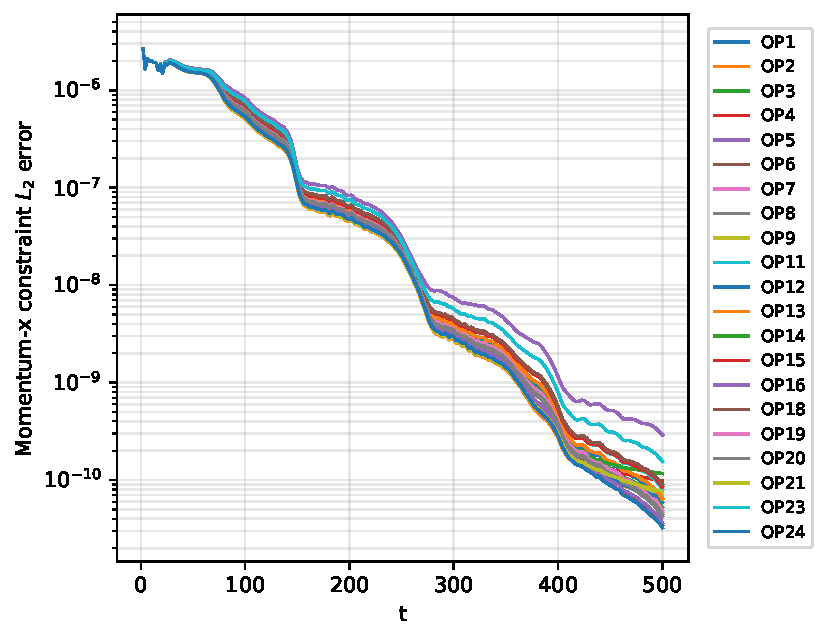
\includegraphics[width=0.9\textwidth]
    {Figures/Appendix/all_momentum_x_errors.pdf}
    \caption{
    Evolution of the momentum constraint error during the Teukolsky wave
    stability test for the finite difference operators considered in this
    work. The computational domain is $x,y,z\in[-40,40]$, and the initial
    data describe an outgoing, even parity Teukolsky wave in the
    $(\ell,m)=(2,0)$ mode with amplitude $\mathcal{A}=10^{-2}$.
    The initial perturbation is centered at $r_0=20$ and uses a compactly
    supported $C^k$ radial profile with $k=6$ and half width $w=2$.
    The errors remain bounded and decay smoothly to small values over more
    than ten characteristic crossing times, with no evidence of a growing
    numerical instability.
    }
    \label{fig:all_momentum_x_errors}
\end{figure}


\section{Black Hole Merger Tests with CFDs}
\label{sec:black_hole_merger_tests}

We also compare the performance of compact and explicit finite difference
operators in an inspiraling equal mass binary black hole merger. The binary
has mass ratio $q=1$, an initial separation of $8M$, and quasicircular initial
data.

We compare evolutions using fourth-order compact and explicit finite-difference operators with a finest resolution of (h=0.0325) against a more highly resolved sixth-order explicit finite-difference evolution with a finest resolution of (h=0.016).

The resulting gravitational waveforms are shown in
Figs.~\ref{fig:bbh_waveforms_overlay} and
\ref{fig:bbh_waveforms_peak_aligned_subtraction}. The fourth order explicit
evolution is underresolved, which produces a noticeable shift in the merger
time. Differences also remain after aligning the waveforms at their peaks.

These results show that the compact operators can outperform explicit
operators of the same nominal order in a fully nonlinear numerical relativity
simulation. In particular, the compact evolution more closely follows the
higher resolution sixth order explicit reference waveform. Further tests are
ongoing to determine how robust these improvements remain across different
resolutions, binary parameters, and longer inspiral evolutions.

\begin{figure}[t]
    \centering
    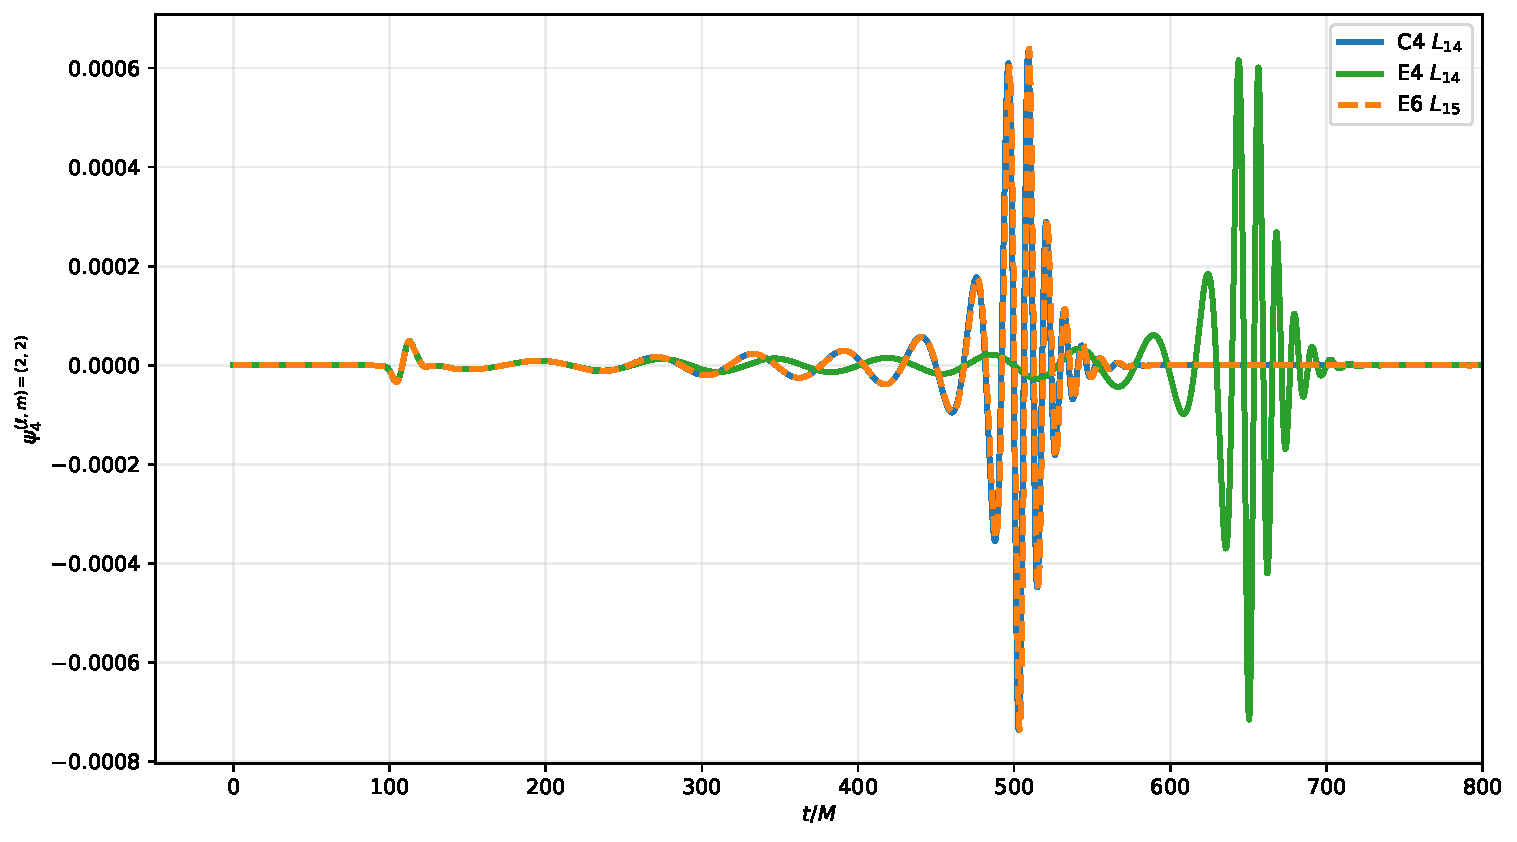
\includegraphics[width=\textwidth]
        {Figures/Appendix/waveforms_overlay.pdf}
    \caption{
    Comparison of the gravitational waveforms from the equal mass binary
    black hole merger evolved with compact and explicit finite difference
    operators. The binary has mass ratio $q=1$, initial separation $8M$, and
    quasicircular initial data. A more highly resolved sixth order explicit
    evolution is included as a reference. The underresolved fourth order
    explicit evolution shows a noticeable shift in merger time, while the
    compact evolution remains closer to the reference waveform.
    }
    \label{fig:bbh_waveforms_overlay}
\end{figure}

\begin{figure}[t]
    \centering
    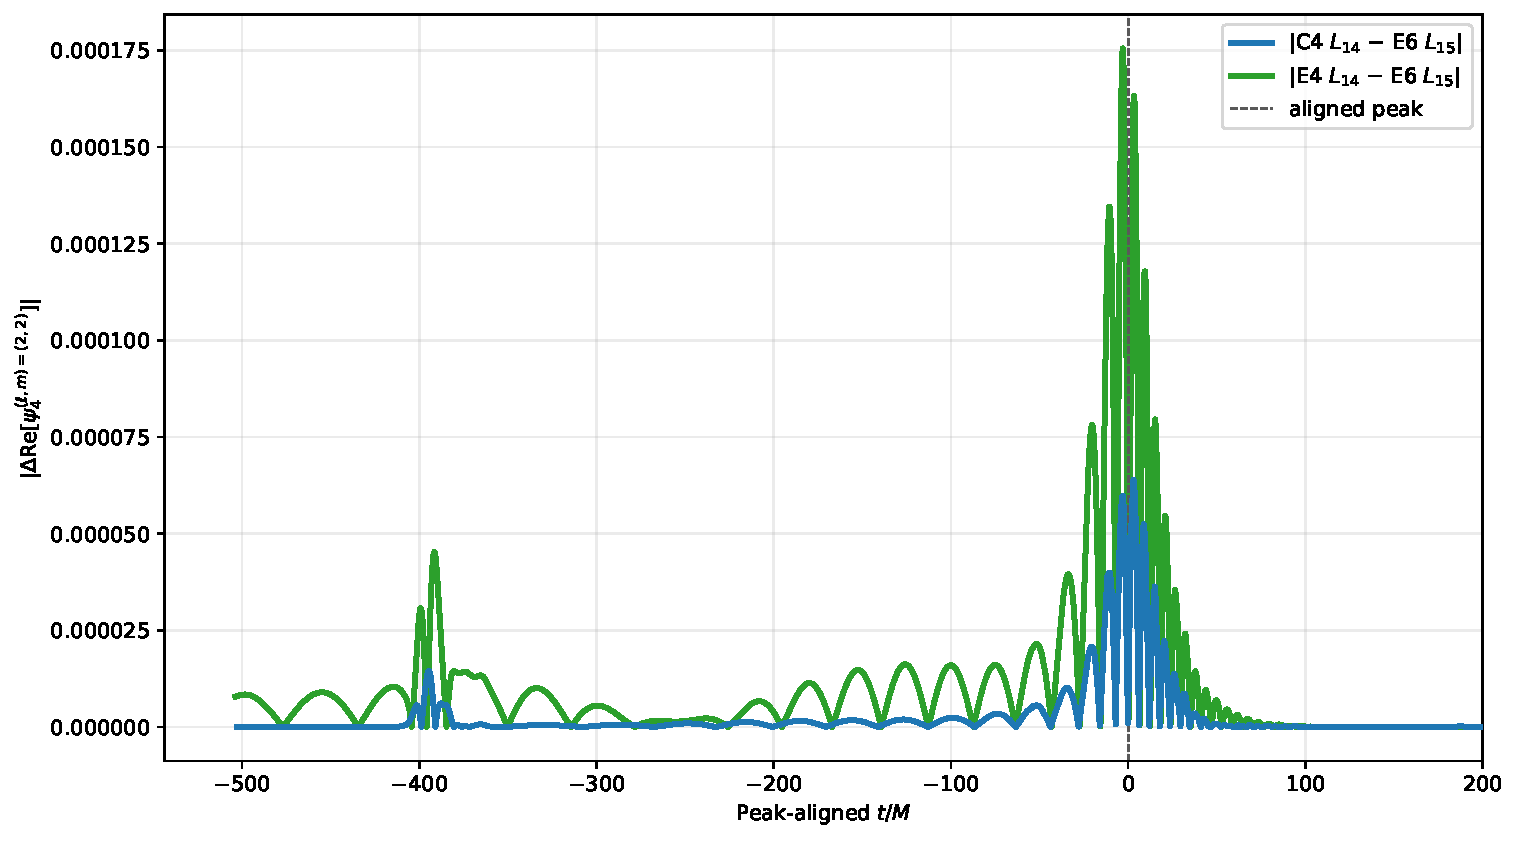
\includegraphics[width=\textwidth]
        {Figures/Appendix/waveforms_peak_aligned_subtraction.pdf}
    \caption{
    Differences between the peak aligned gravitational waveforms from the
    compact and explicit finite difference evolutions and the more highly
    resolved sixth order explicit reference waveform. Peak alignment removes
    the leading merger time offset and highlights differences in waveform
    amplitude and phase. The compact evolution agrees more closely with the
    reference waveform than the underresolved fourth order explicit
    evolution.
    }
    \label{fig:bbh_waveforms_peak_aligned_subtraction}
\end{figure}
